\subsection{pFET MOSFET}

In the previous two sections we introduced how an nFET MOSFET transistor operates in both the sub- and superthreshold regime. As mentioned in chapter \ref{chapter:transistor}, there exists another type of MOSFETs: the pFET transistor. Remember that in a pFET, the doped substrates are inversed. The source and the drain contain free holes as the majority carriers and are therefore of p-type. Both lie within a body with electrons as the majority carriers, the n-well. This n-well is connected to the highest voltage $V_{dd}$. The structure of the pFET is shown in figure \ref{fig:pfet}.\\

\begin{figure}
    \centering
    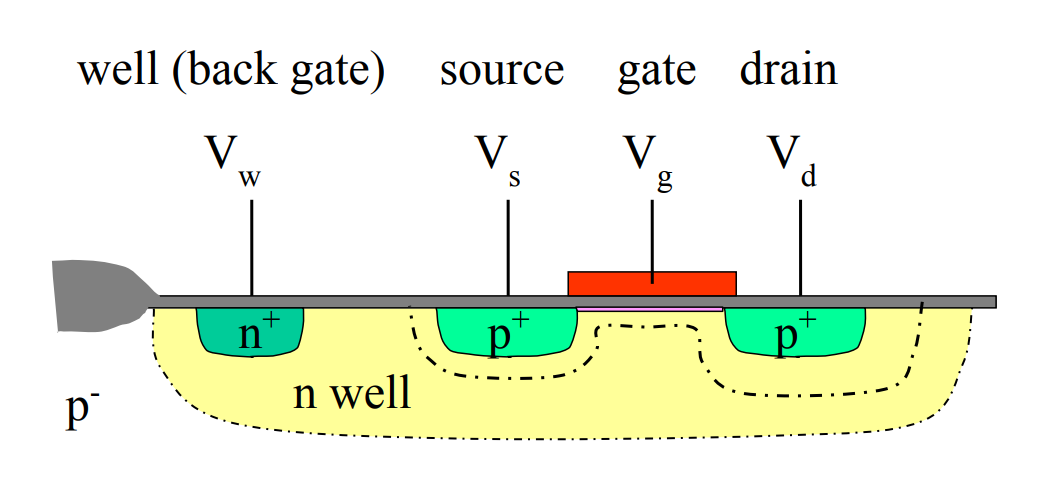
\includegraphics[width=.8\linewidth]{Figures/pFET.PNG}
    \caption{Structure of a pFET MOSFET.}
    \label{fig:pfet}
\end{figure}

The pFET transistor behaves exactly like the nFET transistor but inversed. What exactly does that mean? The transistor is turned off when the gate voltage $V_g$ is at the highest voltage $V_{dd}$. As there is no potential difference between the gate and the n-well, there is no surface potential and hence no current along the channel. When we now decrease the gate voltage of the pFET, the negative potential difference repels the free electrons within the n-well at the surface of the channel and we get a region of fixed positive ions only, the depletion region. As described in the previous section, the diffusion in this region creates a current $I_{sd}$. If we further decrease the gate voltage, free holes eventually become attracted to the channel surface and an inversion region of p-type is created. Similar to the previous derivations, we get the following equations for the current in a pFET MOSFET. Note that they are exactly like the nFET equations but with an inverted sign.\\

\textbf{Superthreshold pFET $I_{sd}$ current}
\begin{itemize}
    \item Triode/ Linear/ Ohmic Region
    \begin{equation}
        I_{sd} = \beta (V_{sg} - |V_T|) V_{sd}
    \end{equation}
    \item Saturation Region
    \begin{equation}
        I_{sd} = \frac{1}{2} \beta (V_{sg} - |V_T|)^2
    \end{equation}
\end{itemize}

\textbf{Subthreshold pFET $I_{ds}$ current}
\begin{itemize}
    \item Triode/ Linear/ Ohmic Region
    \begin{equation}
        I_{sd} = I_0 e^{\frac{-\kappa V_g + V_s}{U_T}} (1 - e^{\frac{V_{ds}}{U_T}})
    \end{equation}
    \item Saturation Region
    \begin{equation}
        I_{sd} = I_0 e^{\frac{-\kappa V_g + V_s}{U_T}}
    \end{equation}
\end{itemize}